\documentclass[12pt]{article}
\usepackage[utf8]{inputenc}
\usepackage[spanish]{babel}
\usepackage{graphicx}
\usepackage{float}
\usepackage{color}
\usepackage{amsmath}
\usepackage{amssymb}
\usepackage[titletoc]{appendix}
\usepackage{vmargin}

\setpapersize{A4}
\setmargins{2.5cm}       % margen izquierdo
{1.5cm}                        % margen superior
{16.5cm}                      % anchura del texto
{23.42cm}                    % altura del texto
{10pt}                           % altura de los encabezados
{1cm}                           % espacio entre el texto y los encabezados
{0pt}               % altura del pie de página
{2cm}              


\title{\textbf{Medición y análisis de la dependencia del campo magnético con la distancia a un imán permanente y a un solenoide.} \vspace{4mm} }

\author{
\textbf{Ernesto Petino Zappala, Ignacio Poggi, Lara Sofía Rosenberg} \vspace{2mm} \\
ernesto.atmo@gmail.com, ignaciop.3@gmail.com, lrosenberg@dc.uba.ar \vspace{2mm} \\
\textit{Laboratorio 3 - Curso de Verano 2017 - Cátedra Bilbao}\\
\textit{Departamento de Física, Facultad de Ciencias Exactas y Naturales, UBA}
}
\date{ }

\begin{document}
\maketitle

\begin{abstract}
Este estudio se enfoca en caracterizar la dependencia del campo magnético con la distancia a distintos tipos de fuentes, y evaluar la aplicabilidad del modelo teórico obtenido de la ley de Ampère. En particular,  se detectó mediante un sensor el campo magnético de un imán permanente de neodimio, y posteriormente el de un solenoide de ($5,0 \pm 0,1$) cm de radio. Del ajuste realizado al campo magnético del imán con respecto a la distancia axial, se obtuvo un momento dipolar $m\approx -0,03$ A$m^{2}$, con $R^2=0,972$. Tanto este ajuste como el correspondiente al campo magnético con respecto a la distancia radial ($R^2=0,994$) comprueban la validez del modelo de dipolo magnético puntual en un rango de distancia de más de 5 cm, aunque es llamativa la diferencia entre el resultado obtenido para $m$ para ambas experiencias, pudiendo ser debida esta a errores de calibración del instrumental. Por otro lado, se ha estudiado el campo magnético de un solenoide real en función de la distancia radial, tanto en su centro de longitud como en un extremo del mismo, dando como resultado una variación notoria del campo en altura pero un alto grado de constancia en desplazamientos radiales.

\end{abstract}

\section{Introducción}

Un campo magnético es un campo vectorial que describe la influencia magnética de las corrientes eléctricas, así como de algunos materiales magnéticos (imanes). \\

Hacia 1820, se descubrió que la circulación de corriente eléctrica estacionaria generaba un campo magnético $B$ con forma circular, cuyas líneas encierran la corriente. Este campo es no electrostático dado que no está generado por carga neta, sino por el desplazamiento de cargas. Se muestra en la ecuación \ref{campo} la expresión de un campo $B$ para una carga única.\\

\begin{equation}
    \textbf{B}=\frac{\mu_0}{4\pi}\frac{(q\textbf{v}\times\textbf{$\hat{u}_r$})}{r^2}
    \label{campo}
\end{equation}

Donde $q$ es la magnitud de la carga, \textbf{v} la velocidad con la que la carga se desplaza, $r$ la distancia radial a la dirección de desplazamiento y $\mu_0=4\pi.10^{-7}\frac{N}{A^2}$ . Esta expresión es conocida como Ley de Ampère. A su vez, un campo magnético generará una fuerza sobre una carga móvil según la ecuación de Lorentz (\ref{lorentz}):

\begin{equation}
    \textbf{F}=q\textbf{v}\times\textbf{B}
    \label{lorentz}
\end{equation}

De esto se deduce que dos cables infinitos paralelos con corriente circulando en sentido opuesto sufrirán una fuerza atractiva (repulsiva si las corrientes circularan en el mismo sentido).
Además, existen materiales llamados imanes permanentes, que tienen la propiedad de conservar su campo magnético una vez que la causa que lo genera ha cesado (al contrario que en el caso regido por la ley de Ampère, donde se requiere la circulación de corriente para que persista el campo magnético).\\
\\
Para facilitar el estudio de los efectos de un campo magnético, suele utilizarse una aproximación llamada dipolo magnético que constituye una aproximación que se hace al campo generado por un circuito por donde circula corriente (o por un imán) cuando la distancia al mismo es mucho mayor a las direcciones del mismo. Los dipolos se pueden caracterizar por una magnitud m llamada momento dipolar magnético, que en el caso de un circuito plano es como se muestra en la ecuación \ref{dipolom} (siendo $I$ la intensidad de la corriente y $S$ la superficie de la espira).


\begin{align}
    \vec{m}=\frac{1}{2}\,I\oint_C \vec{r}\times\vec{dr}=IS\hat{n} 
    \label{dipolom}\\
    \vec{B}(\vec{r})=\nabla\times\vec{A}(\vec{r})=\mu\,\nabla\times\frac{\vec{m}\times(\vec{r}-\vec{r'})}{4\pi\|\vec{r}-\vec{r'}\|^3}
\end{align}

M también puede aplicarse para caracterizar un imán, realizando mediciones a una distancia lo suficientemente grande del mismo.\\

En el caso de un imán cilíndrico de radio $a$,  longitud $L$ y momento dipolar $m$, puede deducirse una expresión simplificada para el campo magnético generado por el mismo sobre un eje $z$ colineal con el eje de simetría del imán a distancias relativamente grandes (varias veces mayores a $a$ y a $L$), que es la siguiente:


\begin{equation}
    \textbf{B}=\frac{\mu_0m}{2\pi z^3}.\textbf{$\hat{z}$}
    \label{campoiman}
\end{equation}

Habiendo medido las dimensiones del imán y tomando varias mediciones del campo magnético generado por el mismo a distintas alturas, puede obtenerse mediante un ajuste estadístico su momento dipolar $m$.\\
\\
La ecuación \ref{br} muestra el campo magnético $B$ en función del radio $r$ con $z$ y $L$ fijos \cite{imanradio}.

\begin{equation}
    B(r)=\frac{\mu_0M}{2}(\frac{z}{\sqrt{z^2+r^2}}-\frac{z-L}{\sqrt{(z-L)^2+r^2}})
    %z=0 fijo!! quizás habría que borrarlo y ya
    \label{br}
\end{equation}

\\

Un dispositivo físico capaz de crear un campo magnético cuasi-uniforme en su interior y muy débil en su exterior se denomina solenoide. Un solenoide ideal será una bobina de hilo conductor enrollado helicoidalmente, de longitud infinita, en cuyo caso el campo magnético en su interior será el de la ecuación \ref{bcte} (siendo $\lambda$ la densidad de espiras por unidad de longitud $\frac{n}{L}$, $\mu_0$ la permeabilidad magnética, $I$ la corriente circulante) y nulo en el exterior.\\

\begin{equation}
    B = \mu_0\lambda I
    \label{bcte}
\end{equation}

Por lo tanto, en un nivel fijo de la longitud de la bobina y a diferentes distancias del centro, el campo magnético debería seguir una función escalón (similar a la función de Heaviside) con $B$ constante para radios menores al radio de la bobina, y nulo para radios mayores.

\section{Dispositivo experimental}

Los instrumentos de laboratorio utilizados fueron:


\begin{itemize}
    \item Sonda Vernier Magnetic Field (rango de medici\'on: 0,32 - 6,4 mT).
    
    \item Conversor analógico-digital Vernier SensorDAQ conectado a una PC mediante el programa MotionDAQ
    
    \item Im\'an cil\'indrico de neodimio, de radio a = (0,580 $\pm$ 0,001) cm; largo L = (0,503 $\pm$ 0,001) cm
    
    \item Bobina de 32,8 $\pm$ 0,1 cm de largo; 5,01 $\pm$ 0,001 cm de radio.
    
    \item Soportes met\'alicos.
\end{itemize}


En primer lugar, se realiz\'o la calibraci\´on de la sonda para calcular el offset de la misma (desplazamiento respecto al 0), mediante el programa MotionDAQ. En la Tabla \ref{tab:calib_sonda} se muestran la f\'ormula utilizada en el programa y los valores obtenidos para los dos rangos permitidos:

\begin{table}[h!]
\centering

\begin{tabular}{|c|c|}
\hline
\multicolumn{2}{|c|}{$B = K_{1}*Tension + K_{0}$} \\ \hline
Rango: 0 - 0,32 mT                       & $K_{0}$ = $-$6,91                  \\ \hline
Rango: 0 - 6,4 mT                  & $K_{0}$ = $-$7,9                  \\ \hline

\end{tabular}
\caption{Valores obtenidos del offset $K_{0}$ de la sonda. $K_{1}$ = 3,225 para ambos rangos.}
\label{tab:calib_sonda}
\end{table}

    
Para hallar el campo magn\'etico $\vec{B}$ del im\'an a lo largo de su eje central (eje \textbf{z}), se coloc\'o el mismo sobre la mesa y por encima la sonda en posici\'on vertical junto a una nuez y al soporte, permitiendo ajustar su altura sobre dicho eje.\\
\\
Al medir $\vec{B}$ a lo largo del radio del im\'an, se utiliz\'o la misma configuraci\'on anterior con una leve modificaci\'on: se fij\'o la sonda a una altura de (7,5 $\pm$ 0,1) cm en el rango de mayor sensibilidad (0 - 0,32 mT); desplazando el im\'an a lo largo de su di\'ametro (con el 0 en el centro del mismo) para obtener los datos correspondientes (Figura \ref{fig:iman_ejes}).

\begin{figure}[H]
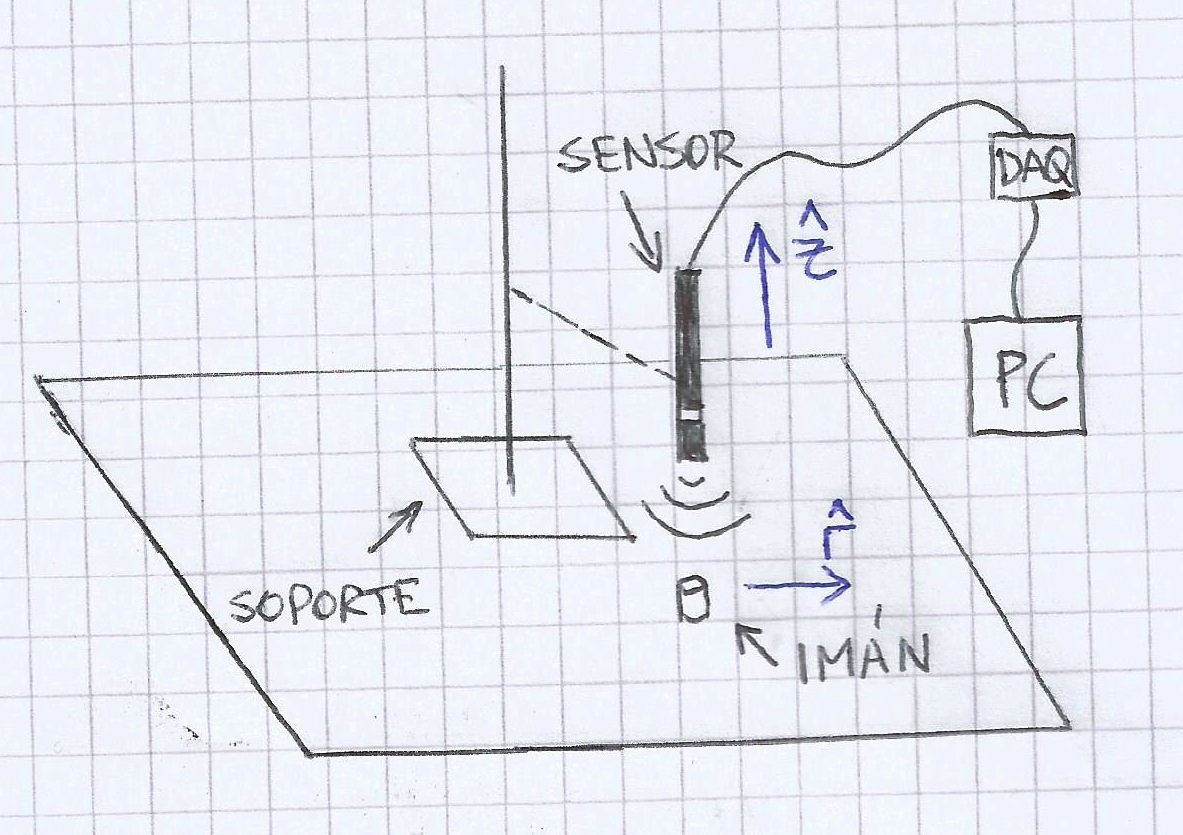
\includegraphics[scale=0.3]{iman_ejes.jpg}
\centering
\caption{Esquema del dispositivo armado para medir el campo magn\'etico del im\'an. En azul, los ejes utilizados en cada experiencia.}
\label{fig:iman_ejes}
\end{figure} 

Para el caso de la bobina se le hizo circular una corriente continua y constante de 194 mA, y se midi\'o el campo magn\'etico dentro y fuera de la misma, fijando la sonda a dos alturas predeterminadas (en nuestro caso, el extremo superior y la parte media de la bobina); y desplazando la sonda a lo largo del di\'ametro del solenoide (con el 0 en el centro del mismo) para obtener los datos correspondientes a $\vec{B}$ (Figura \ref{fig:bobina_ejes}).

\begin{figure}[H]
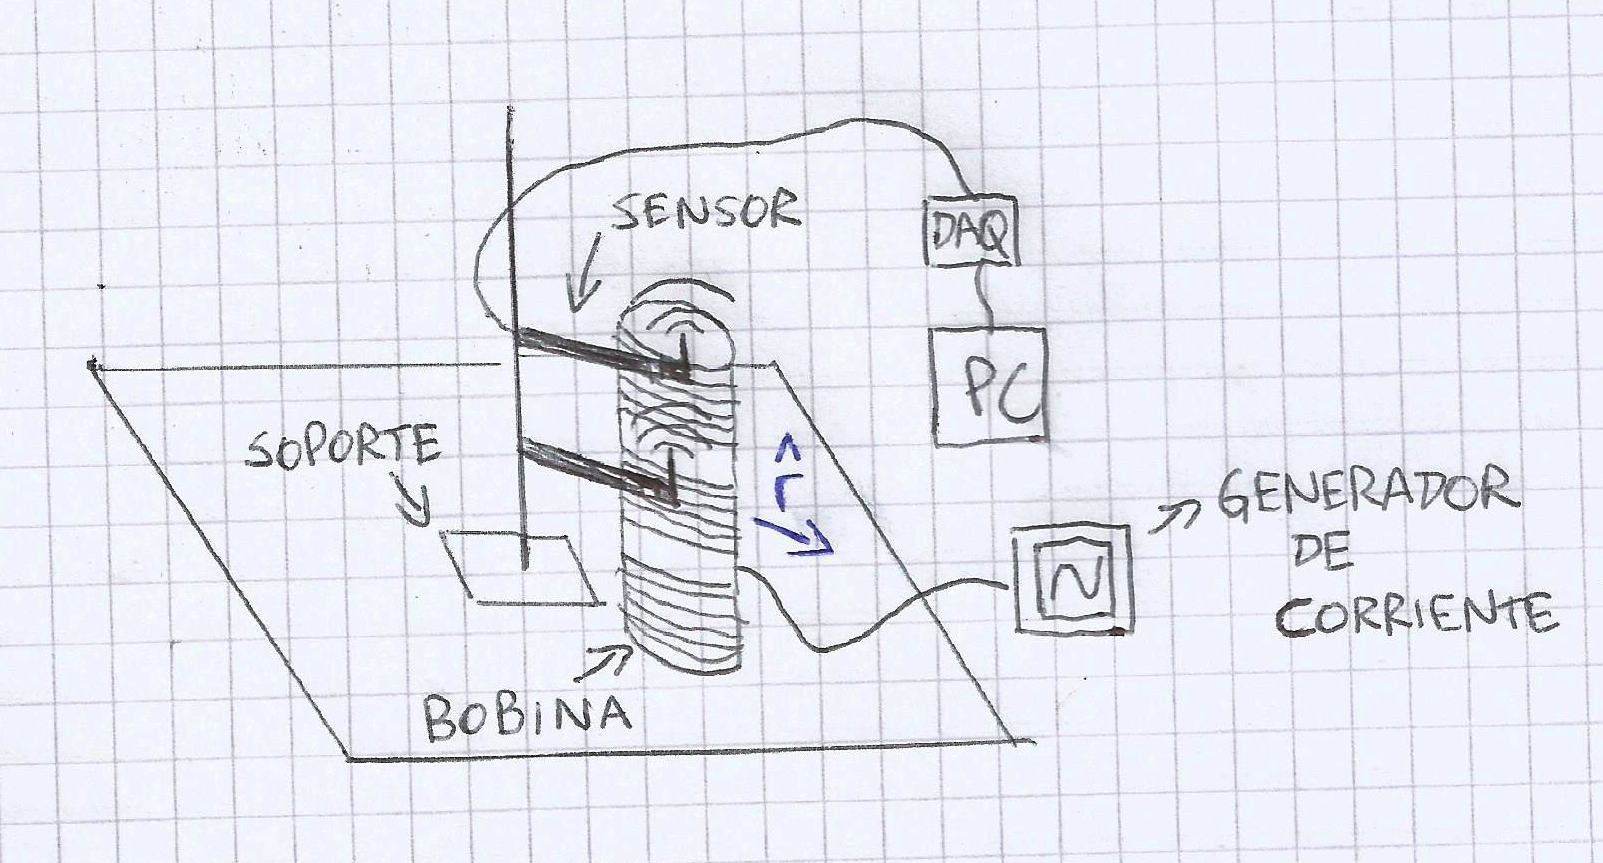
\includegraphics[scale=0.25]{bobina_ejes.jpg}
\centering
\caption{Esquema del dispositivo armado para medir el campo magn\'etico dentro y fuera de la bobina. Se muestran las dos posiciones fijadas del sensor en cada experiencia. En azul, el eje utilizado.}
\label{fig:bobina_ejes}
\end{figure} 



\section{Resultados y an\'alisis}

\subsection{Im\'an}

Al graficar el campo magn\'etico registrado por la sonda en funci\'on de la altura en el eje \textbf{z} definido, se puede observar que a menor altura, el campo magnetico es más intenso. Se tomó como límite inferior un z $\approx$ 5 cm, que corresponde a la validez de la ecuación \ref{campoiman} con las características del imán utilizado (radio y altura). Teniendo esto en cuenta, también se puede observar que a mayor altura ($\approx$ 13 cm) el campo tiende a cero, debido a que la intensidad del mismo es menor en este punto (Figura \ref{fig:iman_altura_ajuste.jpg}).\\



\begin{figure}[H]
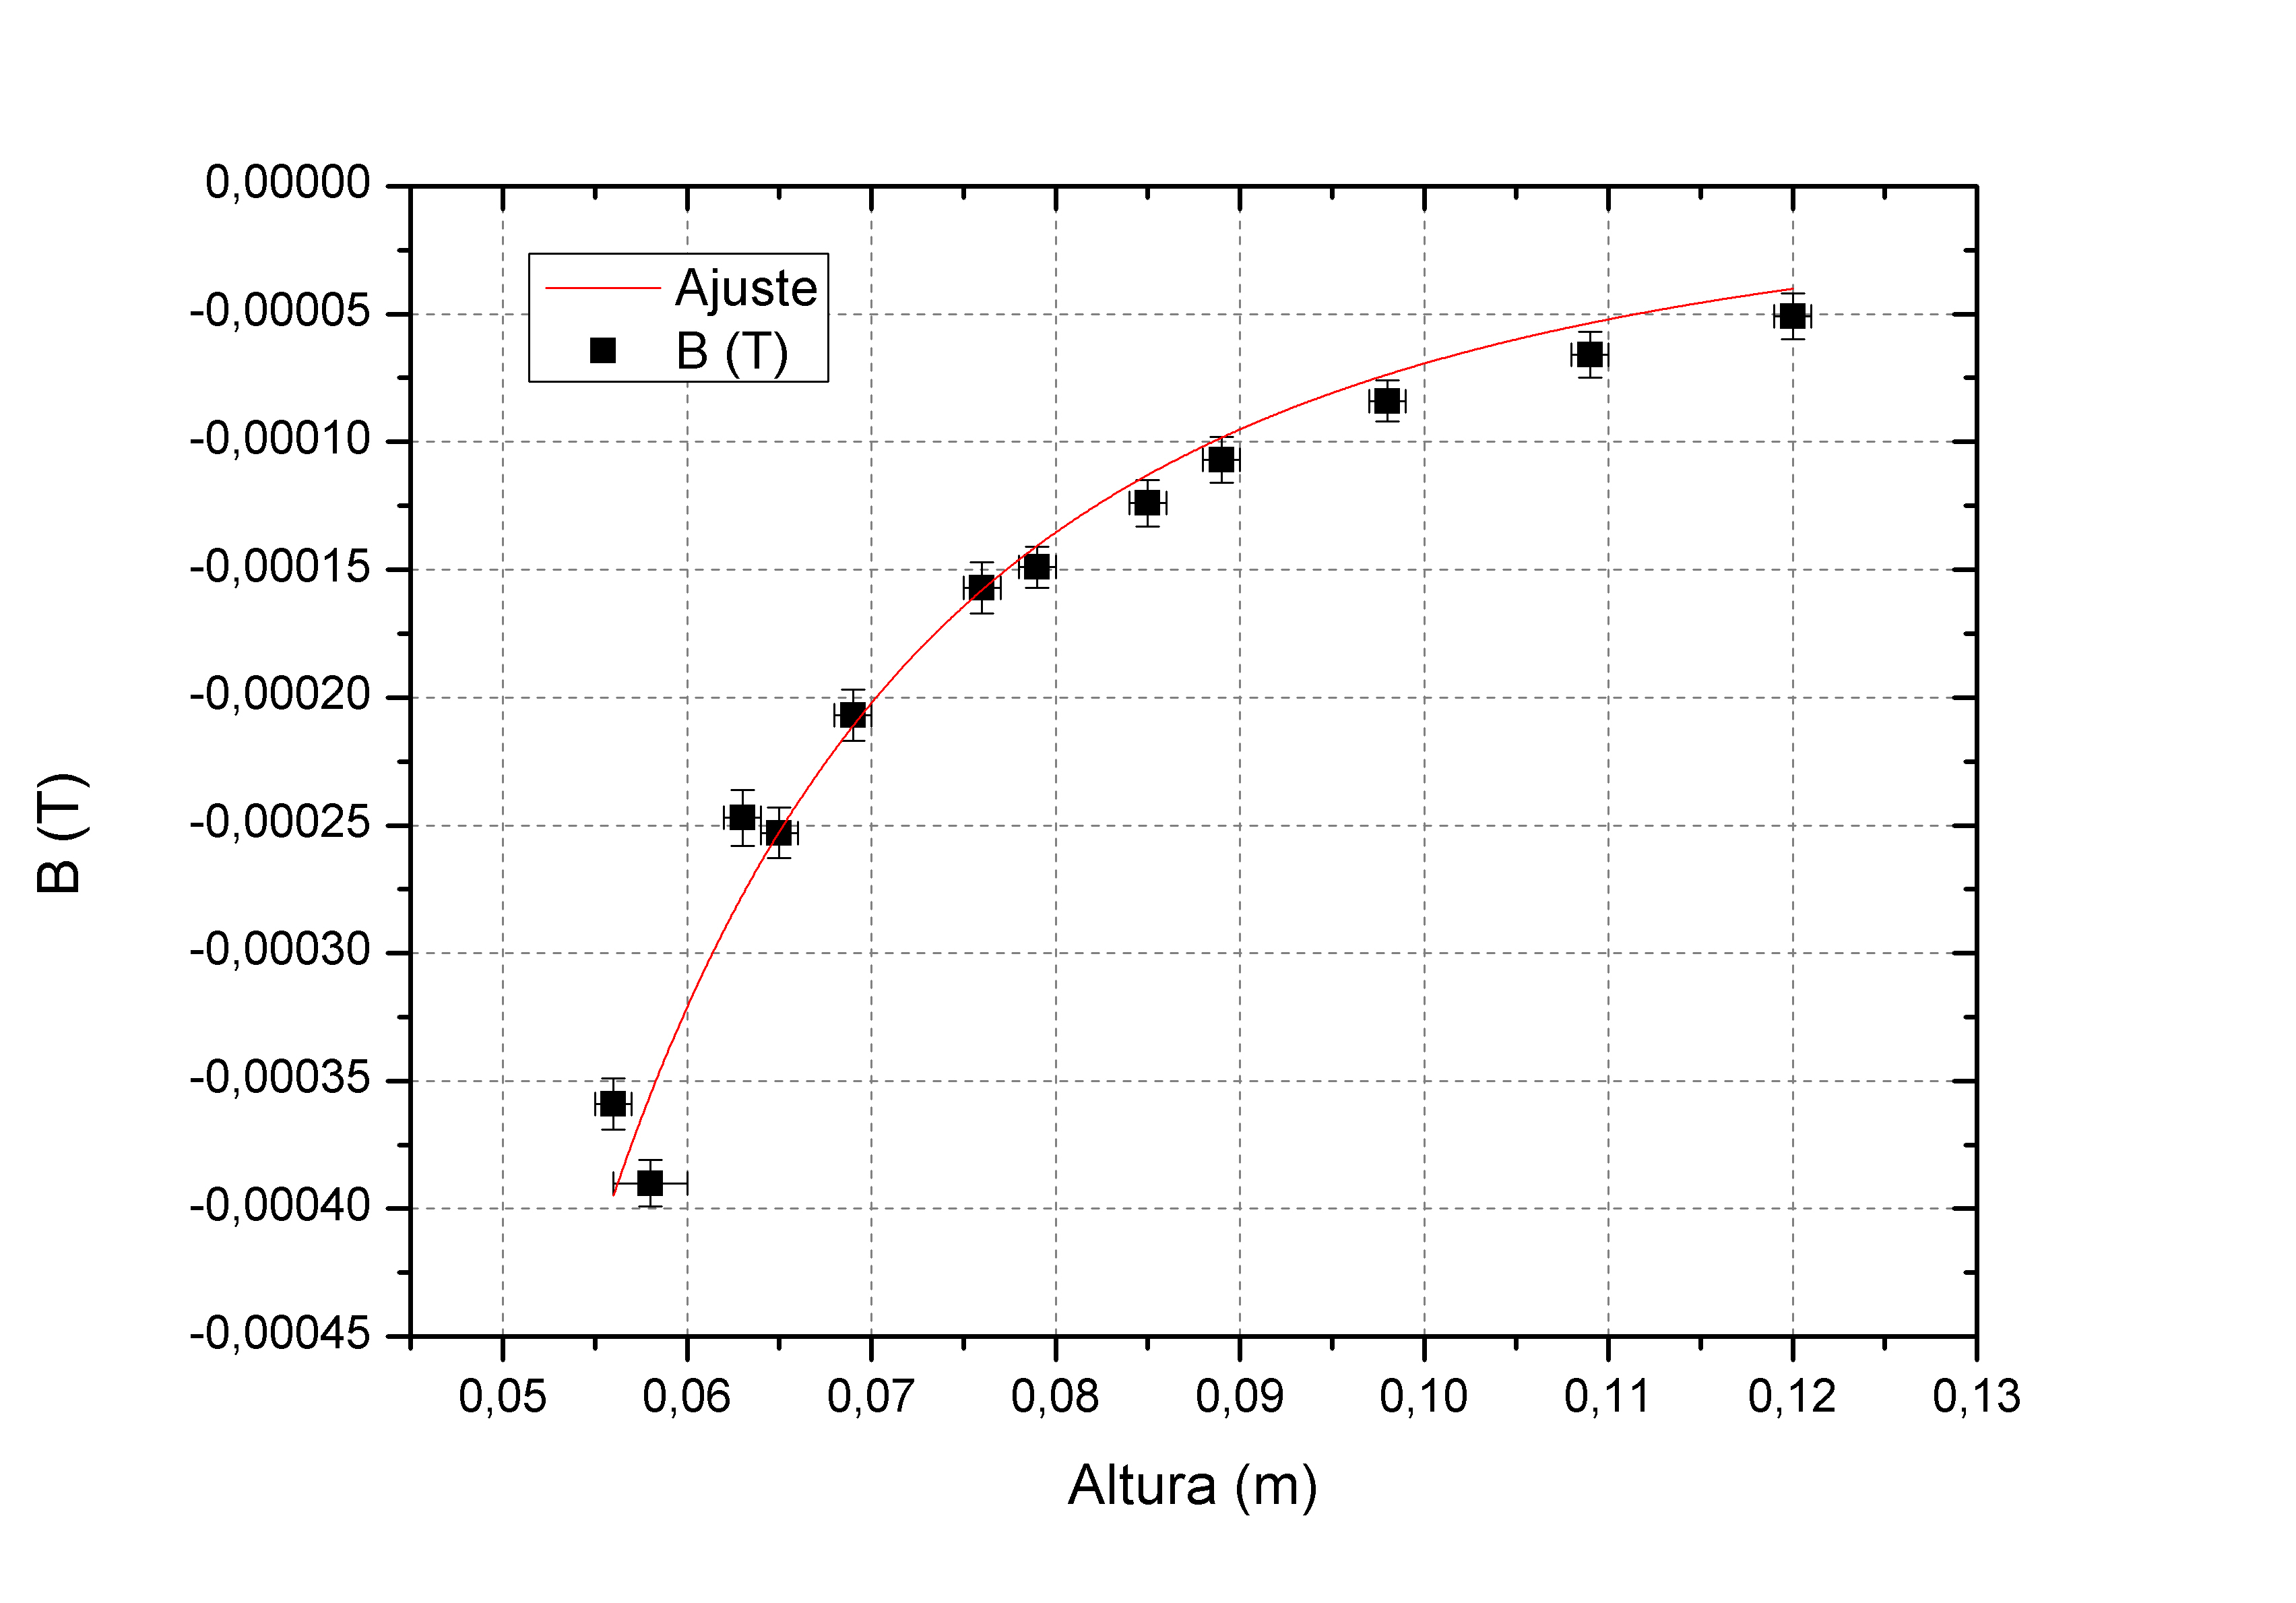
\includegraphics[width=\linewidth]{iman_altura_ajuste.jpg}
\caption{Intensidad del campo magnetico en funcion de la altura. En rojo, el ajuste realizado sobre los datos.}
\label{fig:iman_altura_ajuste.jpg}
\end{figure}

En la tabla \ref{tab:iman_altura_datos} se muestran los par\'ametros obtenidos por el ajuste seg\'un la ecuaci\'on \ref{campoiman} y se estim\'o as\'i que $m\approx -0,03$ A$m^{2}$. El $R^2$ es muy favorable, con lo cual muchos datos son explicados correctamente por el modelo, ademas de que el F-valor obtenido indica que es improbable que el ajuste haya sido aleatorio. El modelo utilizado no present\'o grandes complicaci\'on para ajustar los datos, debido a que la sonda se encontraba en su rango m\'as sensible, y permiti\'o obtener datos m\'as precisos para este caso. \\ 

\begin{table}[H]
\centering
\caption{Ajuste realizado para obtener el momento magnetico en el iman sobre el eje z definido.}
\label{tab:iman_altura_datos}
\begin{tabular}{|c|c|}
\hline
\multicolumn{2}{|c|}{$B(z) = \frac{\mu_{0} m}{2\pi z^{3}}$} \\ \hline
$m$                      & $-0,03468\pm9,09*10^{-4}$                   \\ \hline
$R^2$                       & 0,972                              \\ \hline
F-valor                     & 1454,70                             \\ \hline
\end{tabular}
\end{table}

En el gr\'afico de los residuos se puede ver que para valores grandes de altura, las desviaciones son negativas, y se llega a observar que en los primeros valores, donde se observa que no se cumplen las condiciones de la ecuacion \ref{campoiman}, los residuos aumentan (Figura ~\ref{fig:residuos_iman_altura}).

\begin{figure}[H]
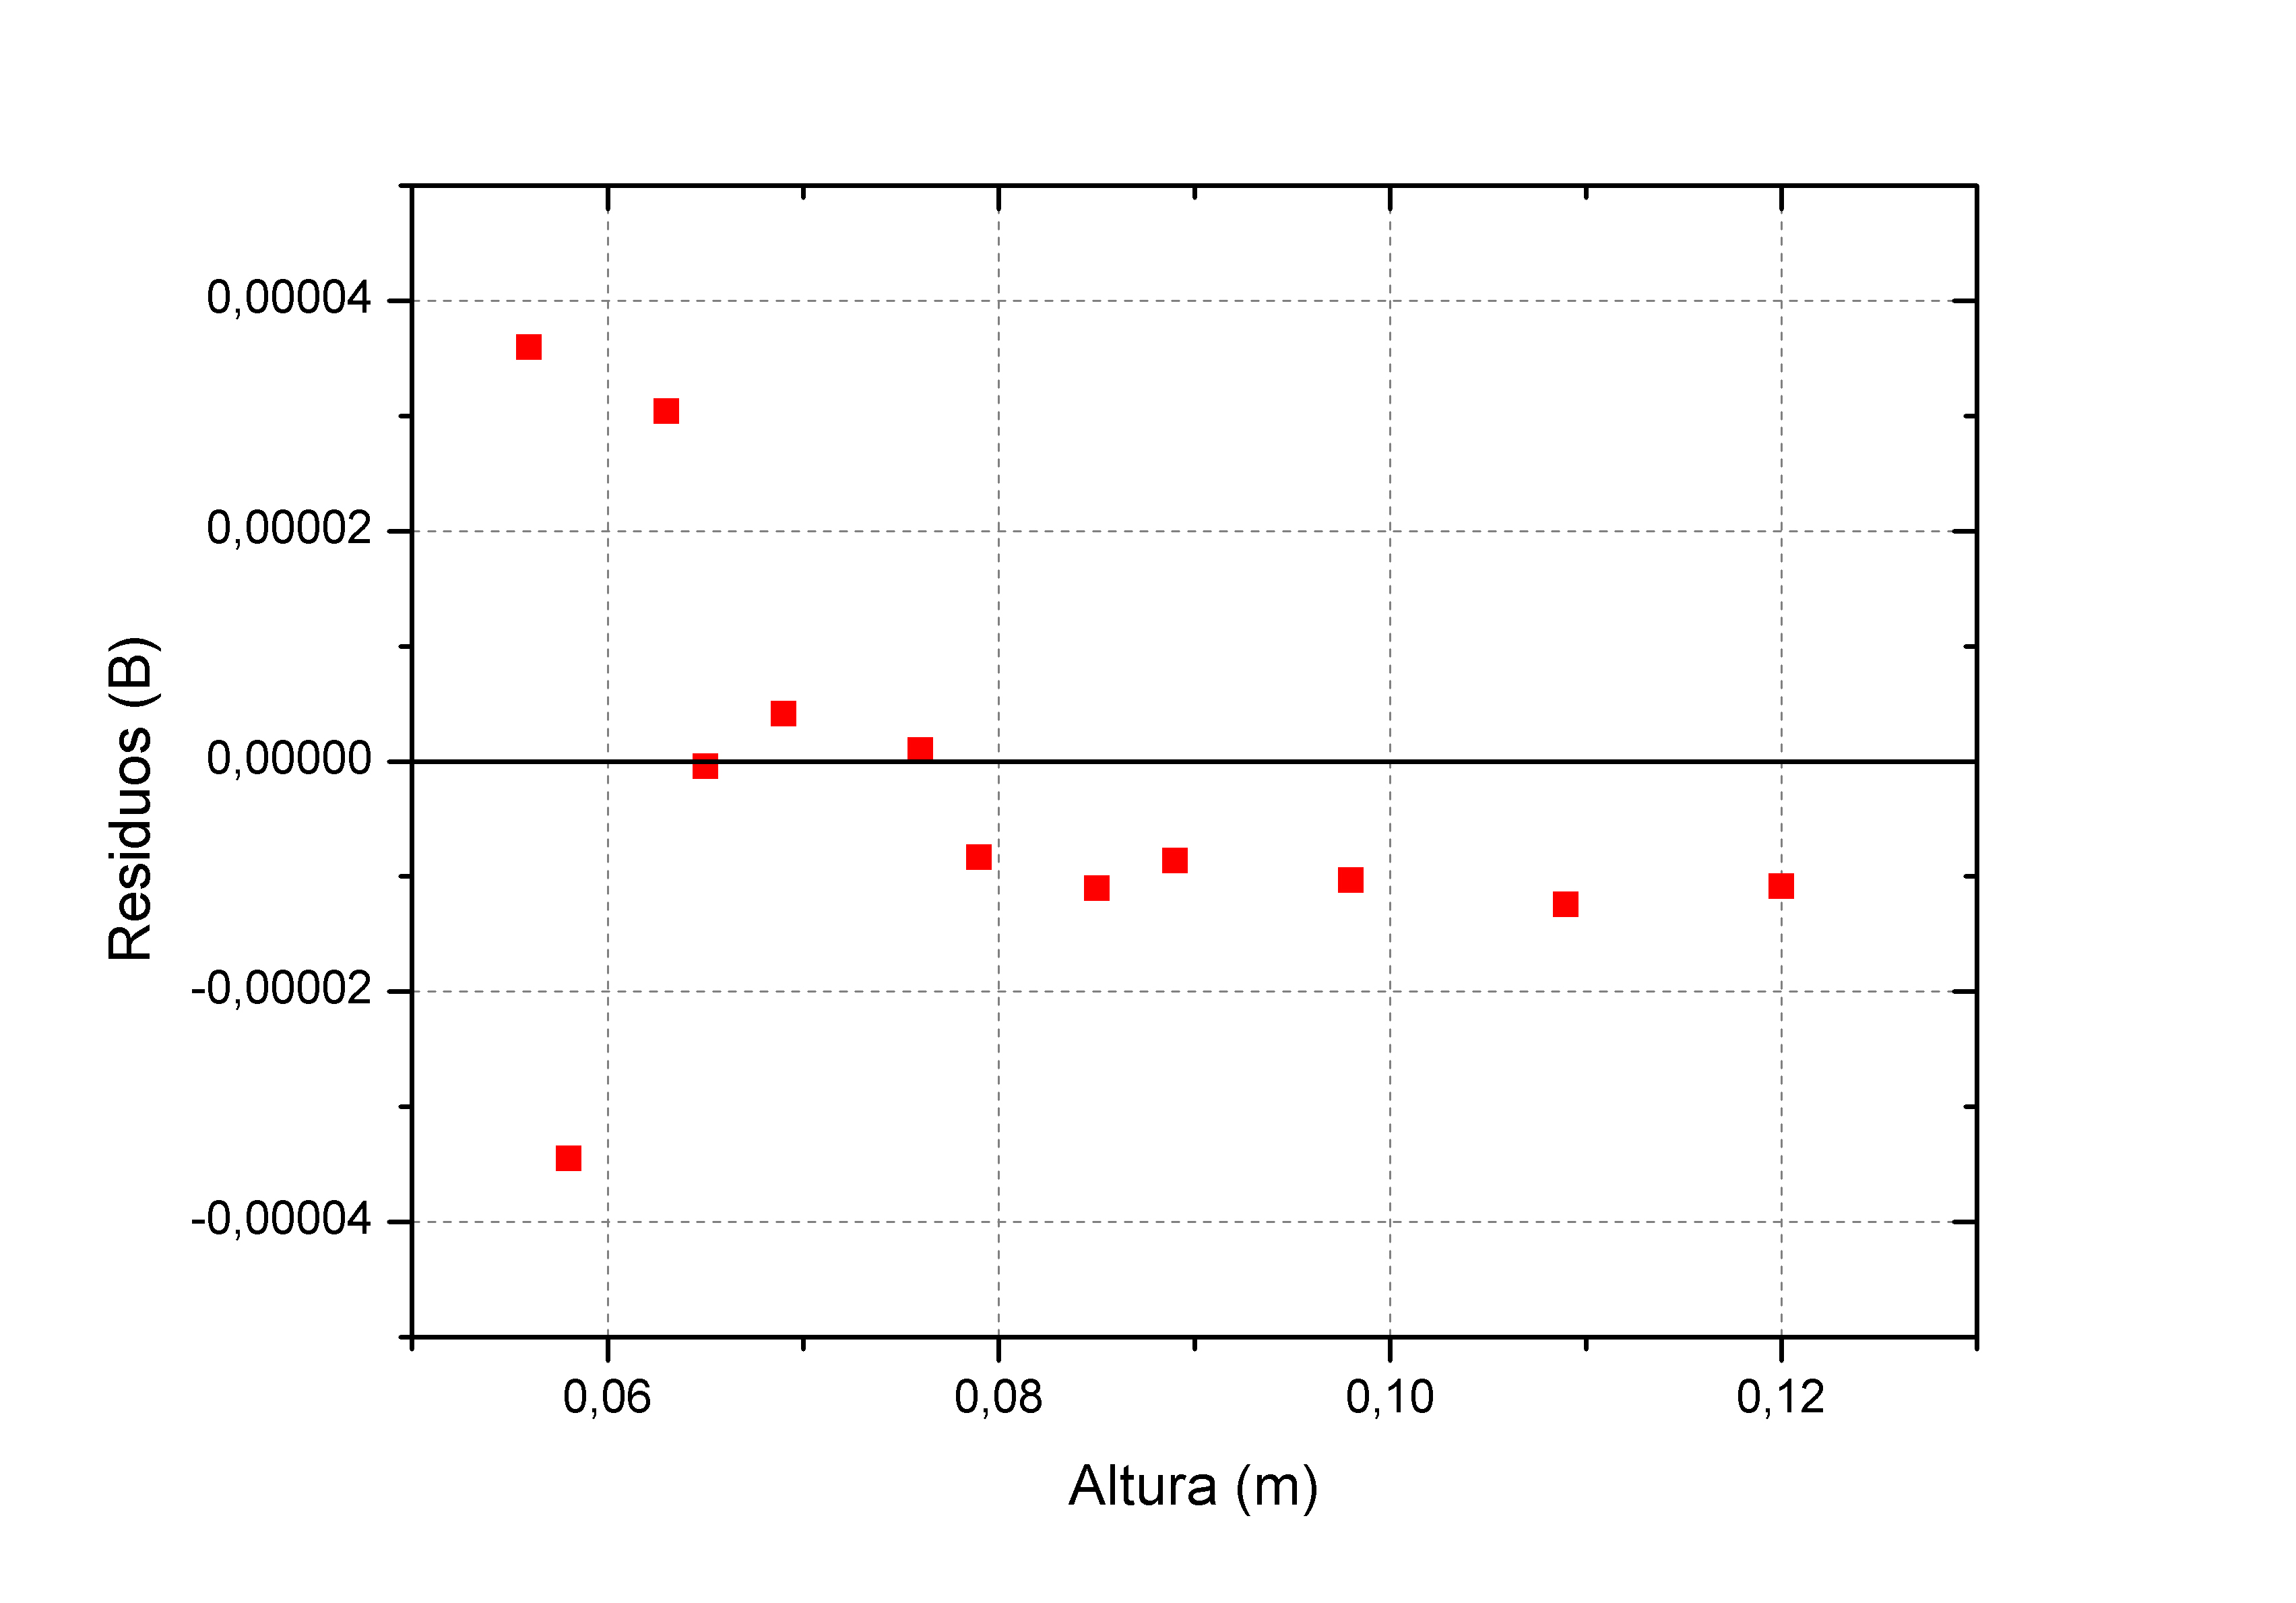
\includegraphics[width=\linewidth]{residuos_iman_altura.jpg}
\caption{Gr\'afico de los residuos obtenidos por el ajuste sobre el eje z definido.}
\label{fig:residuos_iman_altura}
\end{figure}

Tambi\'en se midi\'o la intensidad campo magn\'etico sobre el eje radial del iman. En este caso, se eligio una altura fija para la sonda de 7,5 cm; en la Figura ~\ref{fig:iman_radio_ajuste} se puede observar que en el centro del imán el campo es muy intenso, decayendo a medida que se aleja radialmente la sonda del mismo. Se observó que a más de 10 cm del centro, los valores medidos del campo eran practicamente nulos. Para realizar el ajuste se utilizo la ecuación \ref{br}.

\begin{figure}[H]
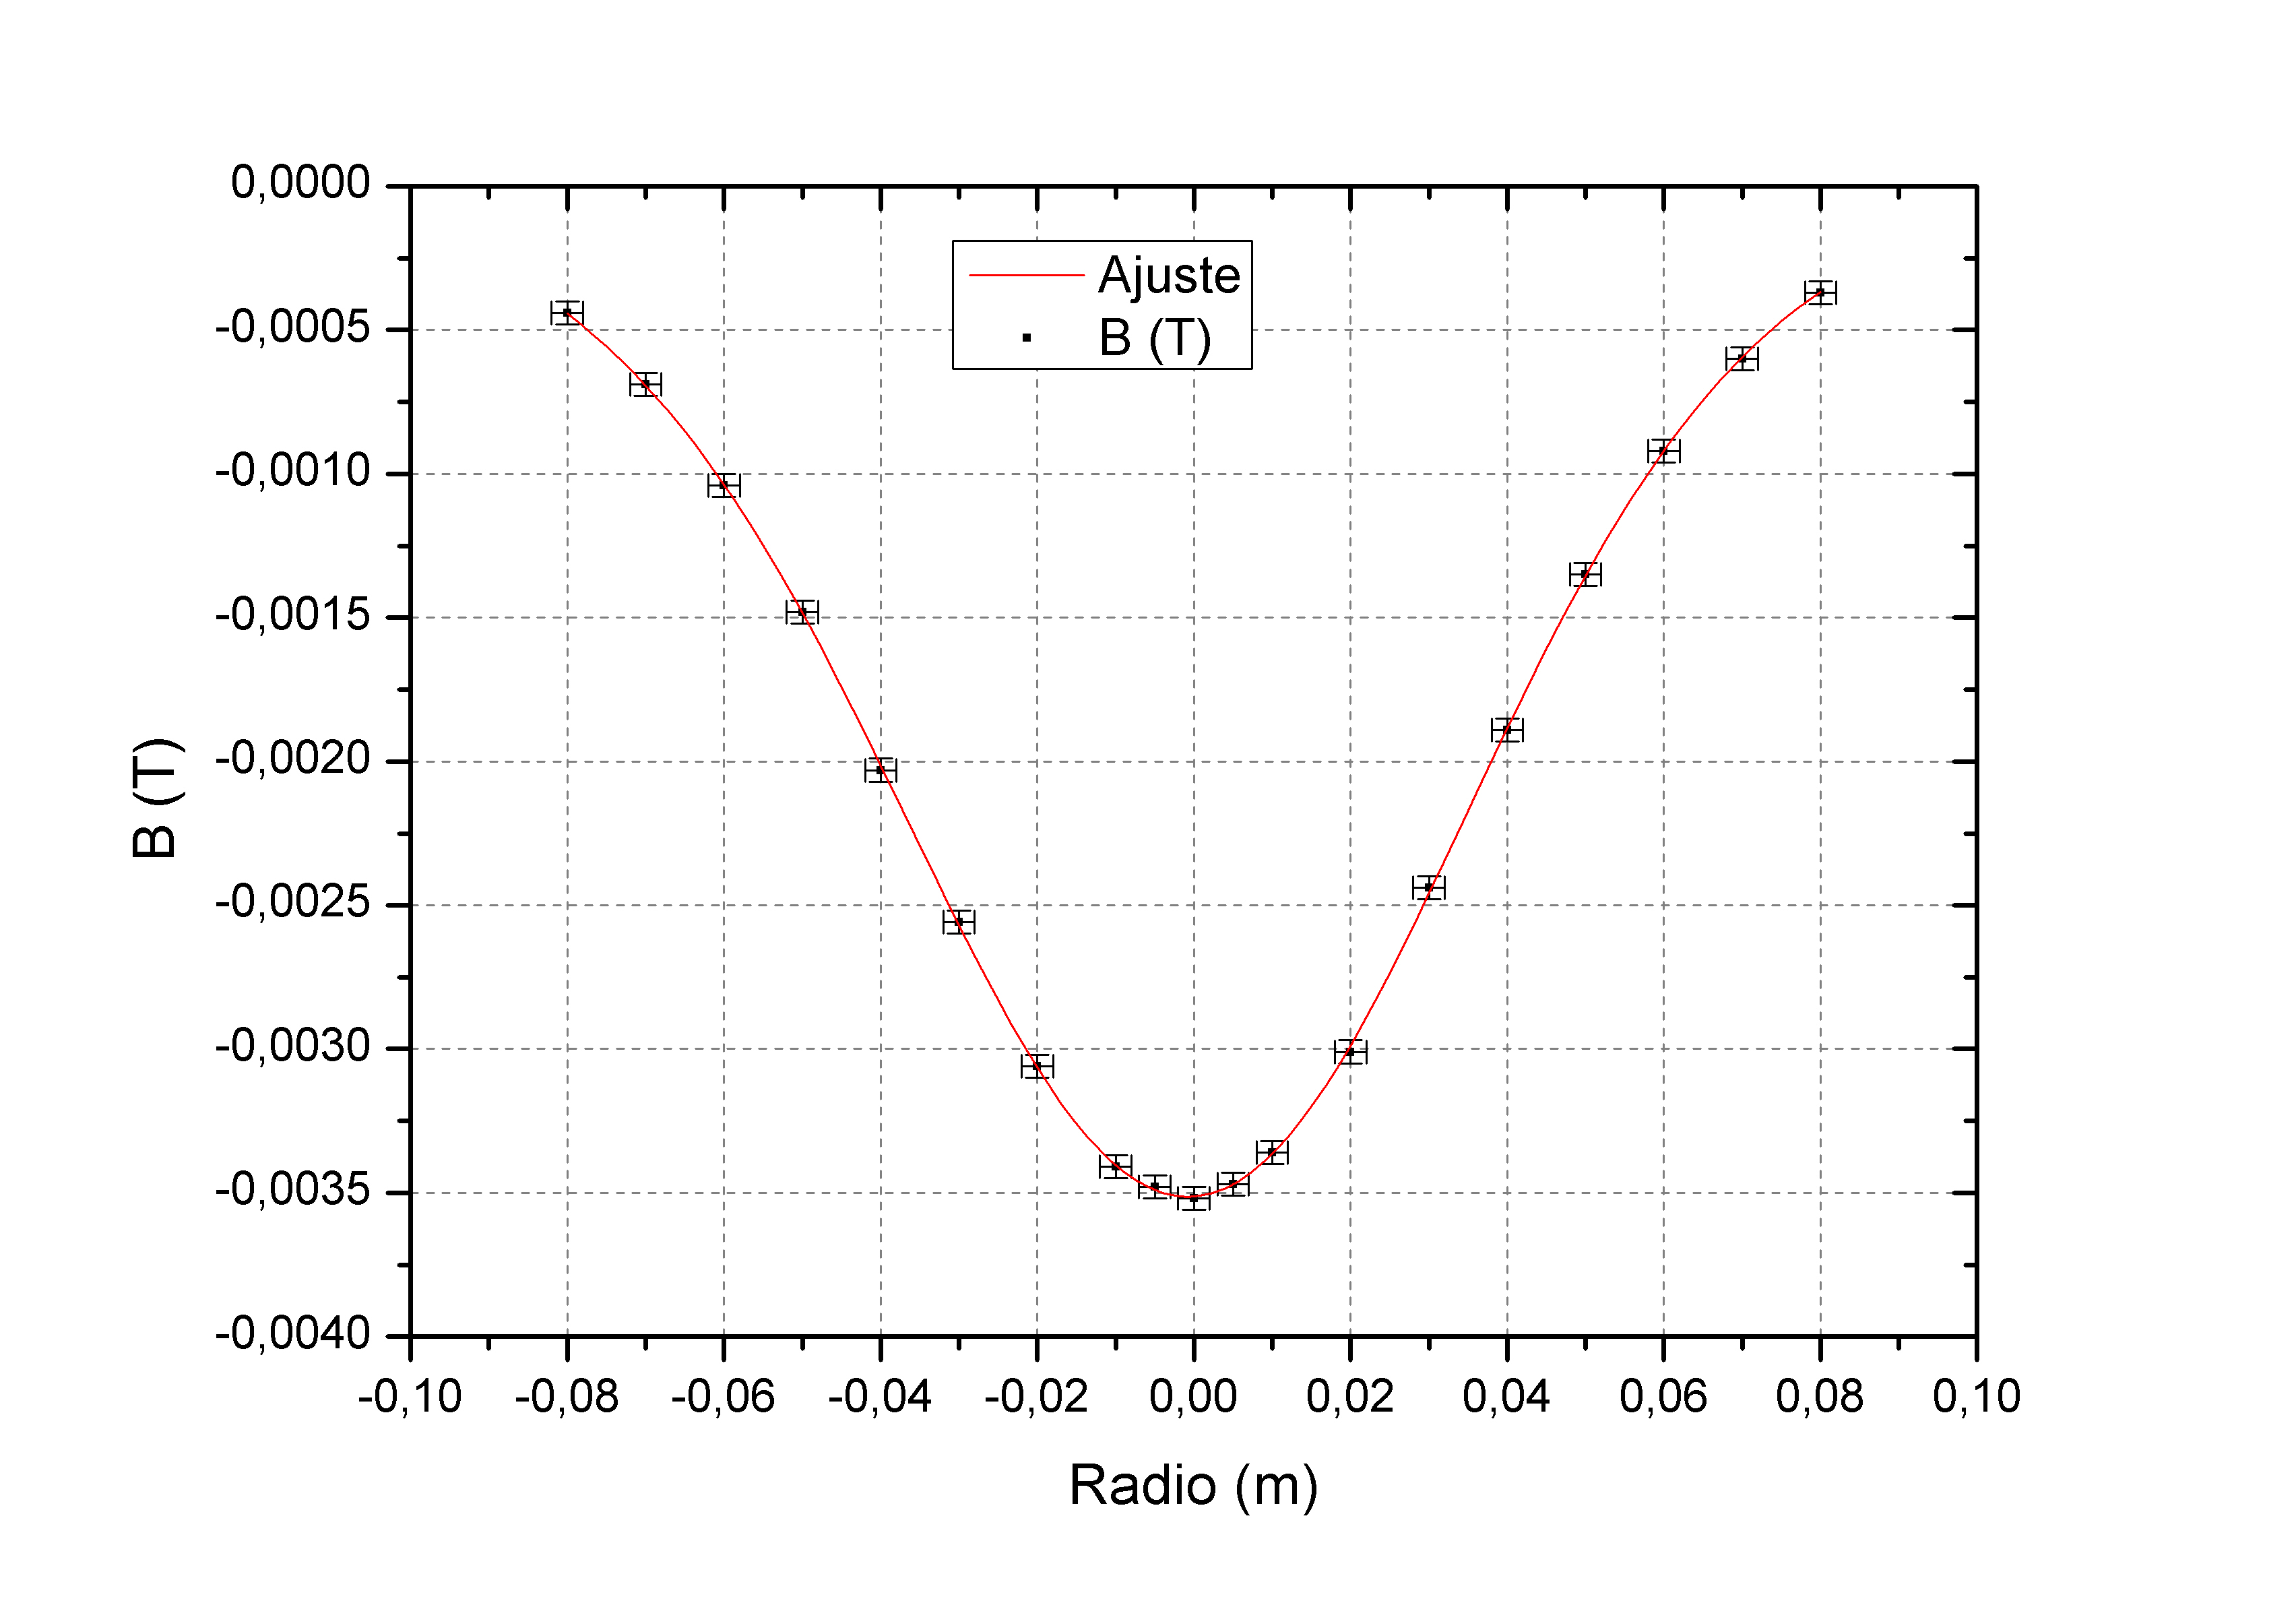
\includegraphics[width=\linewidth]{iman_radio_ajuste.jpg}
\caption{Intensidad del campo magnetico en funcion del radio. En rojo, el ajuste realizado sobre los datos.}
\label{fig:iman_radio_ajuste}
\end{figure}

La tabla ~\ref{tab:iman_radio_datos} muestra los par\'ametros obtenidos por el ajuste seg\'un la ecuaci\'on Y y se estim\'o as\'i que $m\approx -0,02$ A$m^{2}$. El $R^2$ fue mas favorable que en el caso anterior, por lo tanto los datos son explicados correctamente por el modelo, ademas de que el F-valor obtenido tambien fue mucho mayor al obtenido en las mediciones en altura. Para esta experiencia, el modelo utilizado present\'o ciertas complicaciones para ajustar los datos, debido a que la sonda se encontraba en su rango m\'as sensible y al desplazar el iman sobre su eje radial, las mediciones diferian mucho entre valores de radio cercanos. \par 

\begin{table}[H]
\centering
\caption{Ajuste realizado para obtener el momento magnetico en el iman sobre su eje radial.}
\label{tab:iman_radio_datos}
\begin{tabular}{|c|c|}
\hline
\multicolumn{2}{|c|}{$B(r) = Ecuación ~\ref{br}} \\ \hline
$m$                      & $-0,02187\pm8,19*10^{-4}$                   \\ \hline
$R^2$                       & 0,994                              \\ \hline
F-valor                     & 2166                             \\ \hline
\end{tabular}
\end{table}

En este caso, en el gr\'afico de los residuos se observa las desviaciones son uniformes alrededor del 0 para todo el rango de valores del radio, sin embargo se puede observar sutilmente que se ensanchan a medida que se aproximan al 0 (centro del iman), donde el campo es mas intenso. (Figura ~\ref{fig:residuos_iman_radio}).

\begin{figure}[H]
\centering
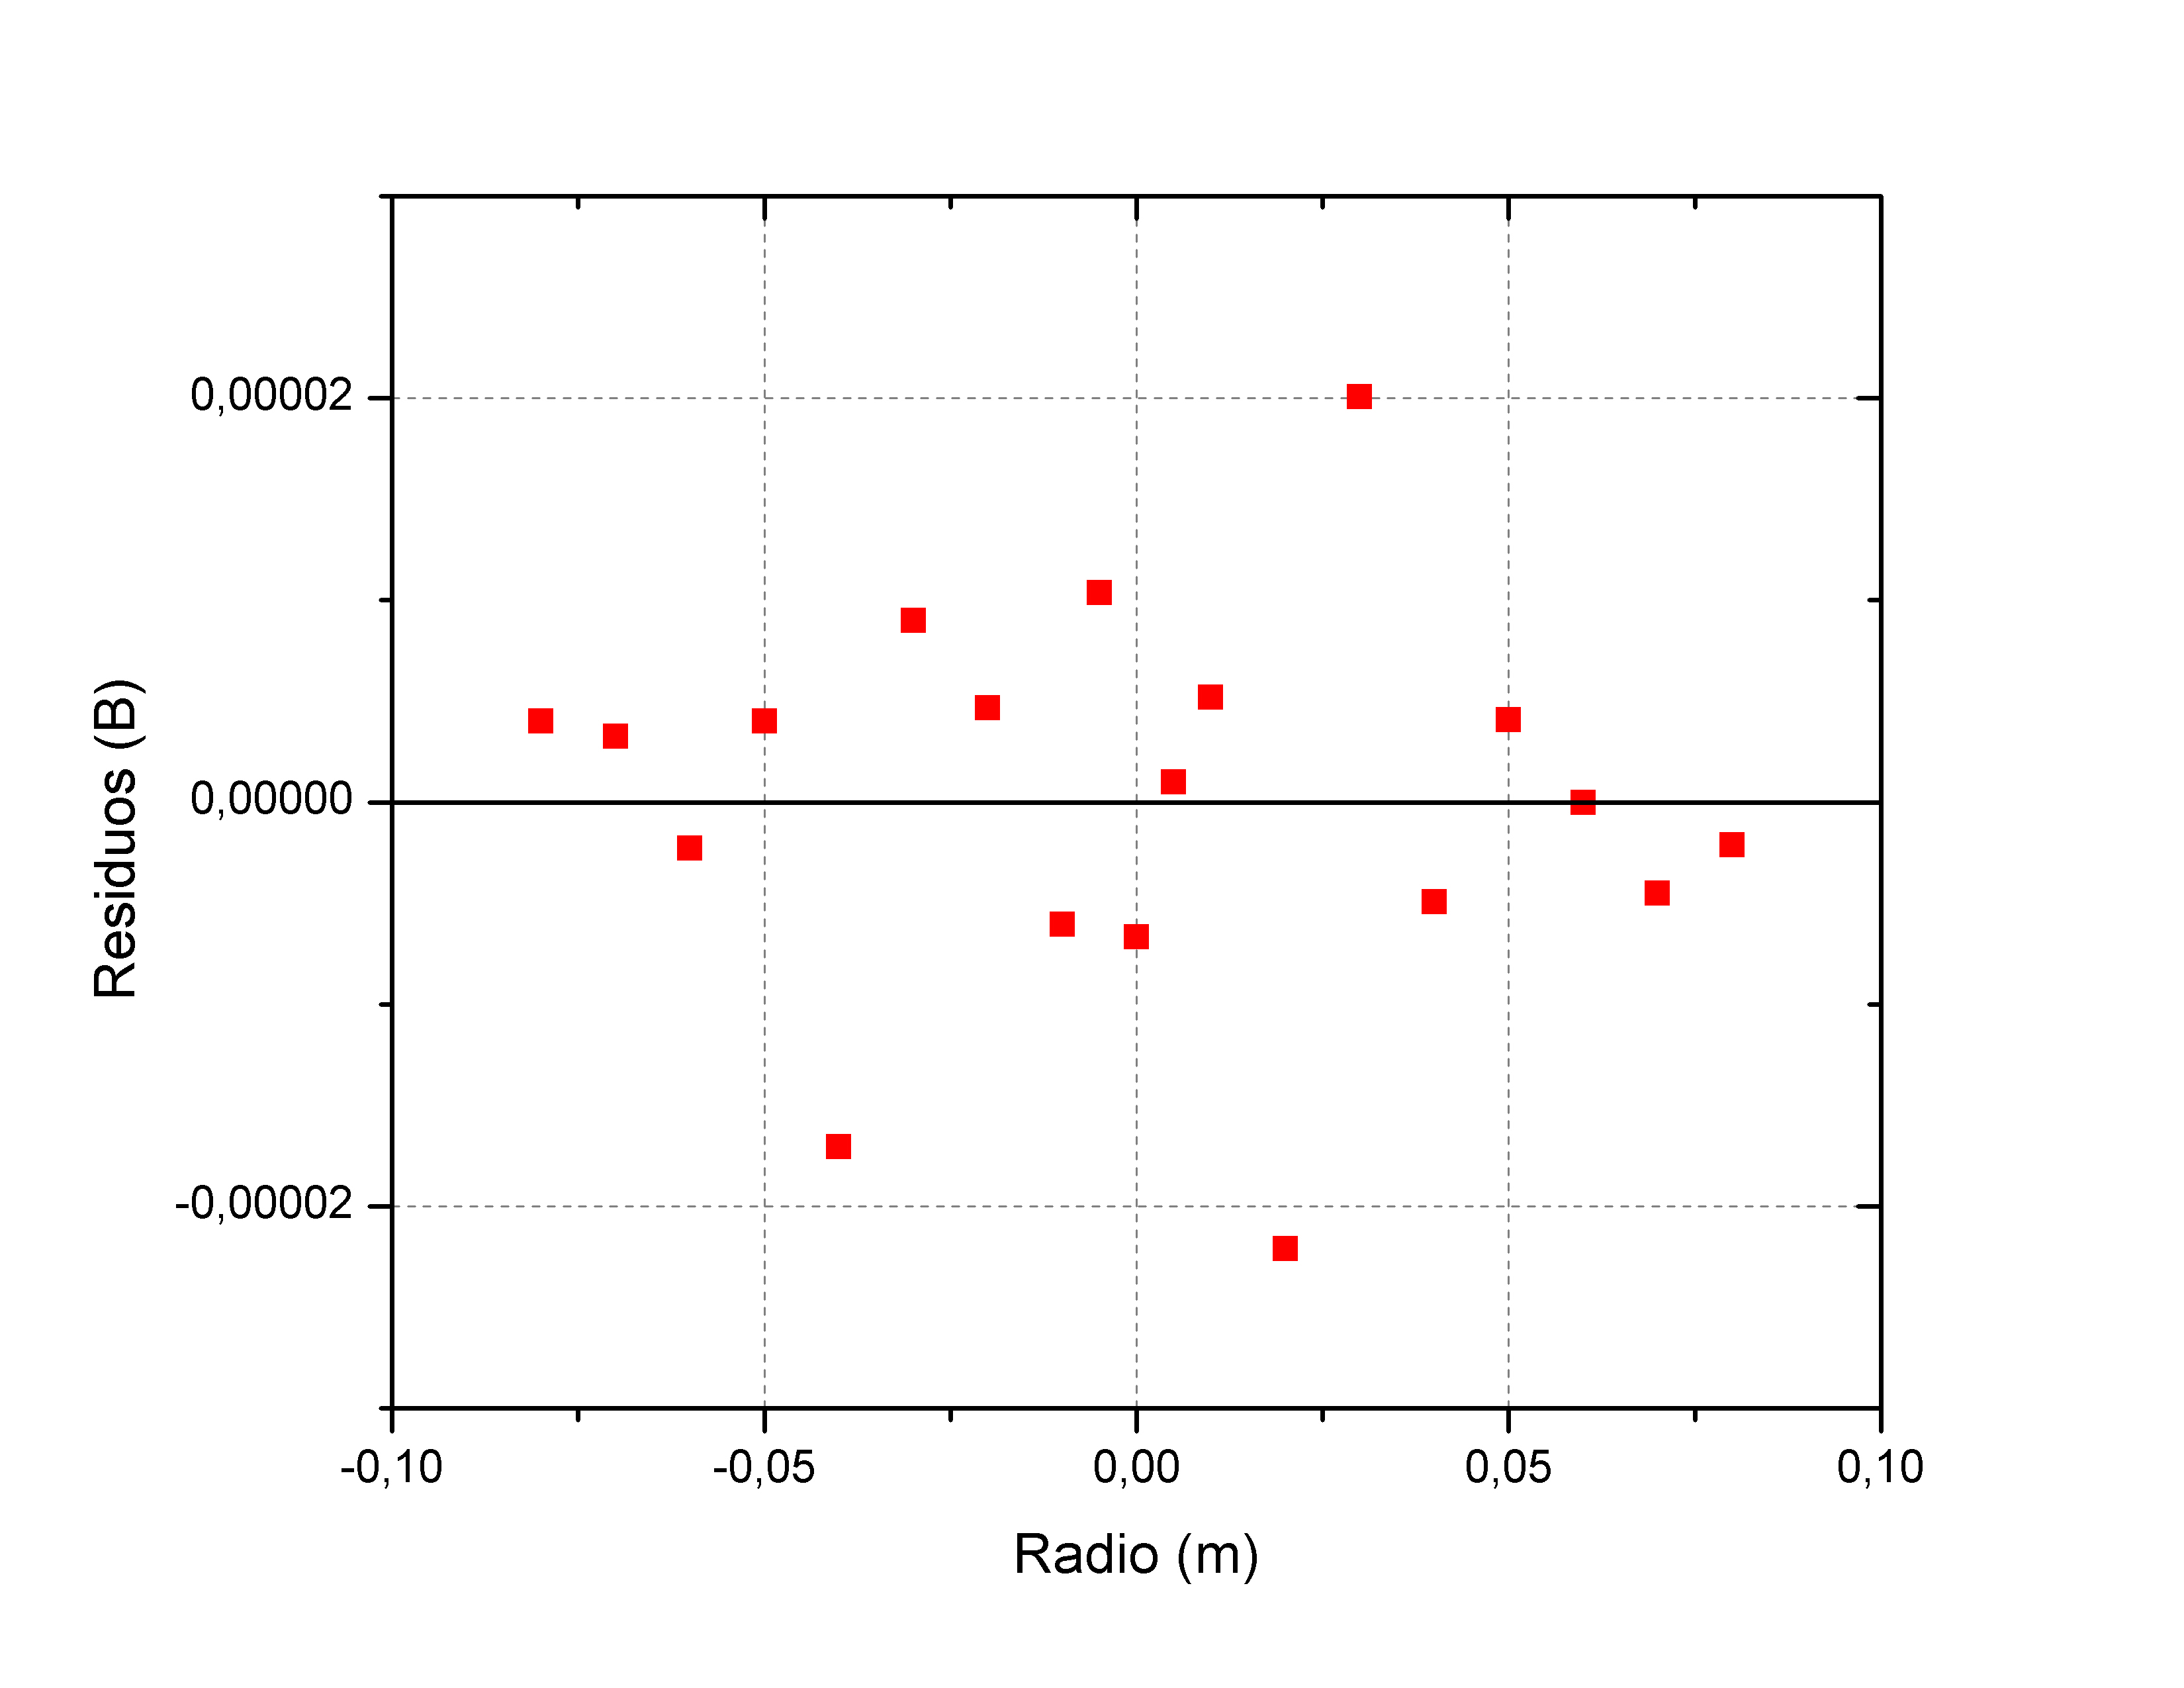
\includegraphics[scale=0.5]{residuos_iman_radio.jpg}
\caption{Gr\'afico de los residuos obtenidos por el ajuste sobre el eje radial.}
\label{fig:residuos_iman_radio}
\end{figure}

Llama la atención la diferencia entre el momento dipolar $m$ obtenido mediante la primera experiencia (medición a lo largo del eje colineal al cilindro) y la segunda (medición a lo largo del eje radial). Esto puede deberse a que para ambas experiencias, se utilizaron distintos niveles de sensibilidad de la sonda. Errores de calibración tampoco pueden ser descartados.


\subsection{Solenoide}

Al medir el campo magnético en el interior y en el exterior del solenoide, variando únicamente la distancia radial en dos series de datos (la primera a $(z=15,9 \pm 0,1)$ cm y la segunda a $(z=31,6 \pm 0,1)$ cm, hallamos una muy buena correspondencia con el modelo propuesto de campo magnético constante en el interior y nulo en el exterior del solenoide.\\ 

En el primer caso, con altura en la mitad del solenoide, se obtuvieron valores distinguibles de campo magnético pero que arrojan un valor central de 0,0003545 T al ajustarlos con una función escalón, disminuyendo a cero a partir de $r=(0,0512 \pm 0,0026)$ cm. Este ajuste por cuadrados mínimos tiene un valor de $R^2=0.991436230697$, con lo cual entendemos que prácticamente todos los datos de la serie son explicados por el modelo. En la figura \ref{solmedio} puede verse el ajuste realizado junto con los datos medidos.\\

\begin{figure}[H]
\centering
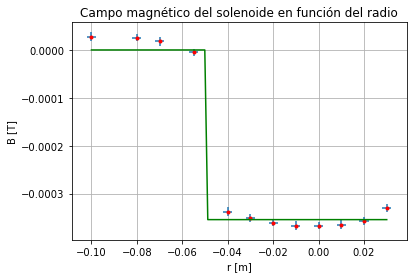
\includegraphics[scale=0.65]{solmedio.png}
\caption{Primera serie de datos de campo magnético vs. distancia radial al centro de la bobina, con altura $(z=15,9 \pm 0,1)$ cm.}
\label{solmedio}
\end{figure}

Asimismo, a partir de este valor de B podemos utilizar la ecuación \ref{bcte} y la corriente entregada al solenoide para estimar su densidad de espiras. Teniendo una corriente de 194 mA, se obtuvo un valor de densidad $n=14,54 \frac{vueltas}{cm}$.\\

Por otro lado, en la segunda serie de datos se obtuvo también una fuerte correspondencia con el modelo teórico, aún estando en el borde del solenoide; es decir, todavía a esa altura rige la aproximación de solenoide infinito en cuanto a la constancia radia del campo. Sin embargo, se observa una disminución del módulo del campo con respecto a la serie de datos anterior, seguramente como efecto de borde. En la figura \ref{solalto} se muestra el ajuste realizado junto con los datos medidos, arrojando un valor central de campo magnético en  -0,002448 T, una caída del campo en $r=(0,0513\pm 0,0025)$ cm -indistinguible de la anterior, y coherente con el radio medido de la bobina-, y un coeficiente $R^2=0,991996454359$. \\

\begin{figure}[H]
\centering
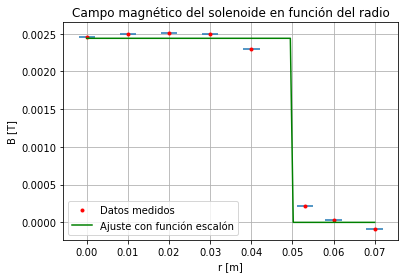
\includegraphics[scale=0.65]{solalto.png}
\caption{Segunda serie de datos de campo magnético vs. distancia radial al centro de la bobina, con altura $(z=32,8 \pm 0,1)$ cm. }
\label{solalto}
\end{figure}

Con esto se comprueba entonces la validez del modelo, que para esta serie de datos estima una densidad de vueltas de  $n=10,04 \frac{vueltas}{cm}$. Nótese que el campo medido en esta altura es positivo, a diferencia del caso anterior. Esto se debe simplemente a que la corriente que se hizo circular por el solenoide tenía sentido opuesto.\\


\section{Conclusiones}

La medición del campo magnético del imán cilíndrico sobre el eje $z$ (colineal al eje del imán cilíndrico) se ajusta bien al modelo de la ecuación (5), con un $m\approx -0,035$ A$m^{2}$ y un $R^2=0,972$, en un rango de distancias entre 5 y 13 cm de distancia al borde superior del imán. Del análisis de los residuos se deduce que el ajuste es peor cerca del imán (apartamientos relativamente grandes entre 5 y 6 cm de altura) y mejor pero con un leve sesgo por debajo de la curva teórica entre los 8 y los 13 cm. La medición sobre un eje radial fijo a una altura de 7,5 cm, en el rango de -10 a 10 cm (ubicándose el 0 sobre el eje de simetría del imán) se ajusta al modelo teórico proporcionado por la ecuación (6) pero obteniendo un $m\approx -0,022$ A$m^{2}$ - menor que en el caso anterior - y un $R^2$ de 0,994, lo que hablaría de un muy buen ajuste. El análisis del residuo es más aleatorio que en el caso anterior, si bien se ve un mayor apartamiento respecto al modelo teórico en las cercanías del eje del imán (entre -4 y 4 cm), debido a la mayor variabilidad del campo con la distancia radial en este rango.\\

Las mediciones del campo magnético en función de la distancia radial al centro de la bobina pusieron en evidencia que el modelo de campo magnético constante para el interior de la bobina y nulo e su exterior, aunque mostraron variaciones notables entre el campo medido en la mitad y en la parte superior del solenoide, debido a que el modelo utilizado es una aproximación de solenoide de longitud infinita. Aún así, se pudo utilizar ambos casos para estimar valores de densidad de espiras del solenoide.\\

\begin{thebibliography}{9}

\bibitem{imanradio}
\emph{Alternative method to calculate the magnetic field of permanent magnets with azimuthal symmetry}, J. M. Camacho y V. Sosa, Revista Mexicana de Física E 59 (2013)


\end{thebibliography}

\end{document}

